\documentclass{scrartcl}
\usepackage[utf8]{inputenc}
\usepackage{hyperref}
\usepackage{url}
\usepackage{natbib}
\usepackage{rotating}
\usepackage{adjustbox}
\usepackage{graphicx}
\usepackage{cleveref}
\usepackage{float}
\usepackage{minted}
\usepackage{xcolor}
\usepackage{listings}

\newcommand{\emailaddr}[1]{\href{mailto:#1}{\texttt{#1}}}

\lstset{
    basicstyle=\small\ttfamily
    breaklines=true, 
    breakatwhitespace=true,
    postbreak=\mbox{\textcolor{gray}{$\hookrightarrow$}\ },
    columns=flexible, 
}


\title{\LARGE
    ChefSync: A Multi-Agent Kitchen Orchestrator
}
\subtitle{Final Report for the Intelligent Systems Engineering Course 2025/26}


\author{
    Fantilli Giorgio \\ \emailaddr{giorgio.fantilli@studio.unibo.it}
}

\hypersetup{
    pdfborder={0 0 0}
}

\date{\today}

\begin{document}

\maketitle

\begin{abstract}
ChefSync is a simulated, grid-based orchestrator designed to manage highly concurrent culinary environments through decentralized multi-agent coordination. The project addresses the complex challenges of modern restaurant kitchens, specifically focusing on dynamic workload balancing, spatial pathfinding, and the resolution of physical resource conflicts. To achieve this, the system enforces a strict architectural dichotomy. The physical layer, implemented in Java, provides a discrete-time 2D spatial simulator that manages environmental state, hardware constraints (workstations), and mutually exclusive resource locks. The logical layer encapsulates the system's intelligence utilizing BDI (Belief-Desire-Intention) agents programmed in Jason and AgentSpeak(L). These autonomous agents---acting as Waiters, Head Chefs, and Station Chefs---communicate via the FIPA Agent Communication Language (ACL). By leveraging the ContractNet Protocol (CNP) for task negotiation, the agents evaluate real-time spatial heuristics and operational availability to effectively orchestrate the decomposition, assignment, and execution of unpredictable order streams.
\end{abstract}

\section*{GenAI Usage Declaration}
During the development of this project and the writing of this report, Generative AI tools were used to assist in tasks such as code formatting, generation of documentation templates, and structural review. All core logic, system architecture, and domain modeling are original work.

\newpage
\tableofcontents
\newpage



\section{Domain \& Core Concepts}

The domain of ChefSync is modeled around the operational dynamics of a professional restaurant kitchen, conceptualized as a highly concurrent, spatially constrained, and unpredictable environment. The kitchen brigade serves as an ideal metaphor for a complex socio-technical system. It requires distributed problem-solving, dynamic workload balancing, and coordination among autonomous entities to achieve a common goal: fulfilling customer orders efficiently.

Unlike a deterministic setup, the kitchen has to deal with constant, unpredictable changes. The agents need to be reactive enough to pick up new tasks as they arrive, but also proactive in navigating the kitchen, sharing workstations, and resolving bottlenecks on their own.

\subsection{The Kitchen Brigade (The Agents)}

Before delving into the technical modeling, it is essential to introduce the actors that populate this environment. The brigade is composed of autonomous agents, each with specific roles, responsibilities, and behaviors:

\begin{itemize}
\item \textbf{The Waiter (1 agent):} The entry point of the system. The Waiter acts as a simple interface with the external environment, injecting a predefined sequence of orders into the kitchen.
\item \textbf{The Head Chef (1 agent):} The central coordinator of the kitchen. The Head Chef receives macro-orders from the Waiter, decomposes them into actionable atomic sub-preparations, and delegates these tasks to the available Station Chefs. It monitors the completion of these sub-preparations to assemble the final dish.
\item \textbf{The Station Chefs (N agents):} The workforce of the kitchen. These agents perform the physical labor. They navigate the kitchen grid, acquire necessary physical resources (workstations like stoves or prep counters), execute the assigned sub-tasks, and report back to the Head Chef upon completion or failure.
\end{itemize}


\subsection{Core Domain Entities}

To abstract the physical kitchen into a computable Multi-Agent System (MAS), the domain is formalized around three primary entities:

\subsubsection{Orders as BDI Goals}
Orders represent requests for dishes injected into the system. From a MAS perspective, rather than passive environmental stimuli, orders are represented as high-level goals. They are initiated by the Waiter agent and communicated to the Head Chef agent via FIPA ACL messages. An order represents a macro-goal that needs to be satisfied, representing a complex workflow that must be orchestrated and synchronized to guarantee correct and timely service.

\subsubsection{Recipes and Task Decomposition}
In this domain, a recipe represents the declarative knowledge of how a macro-goal (a dish) is decomposed into atomic sub-goals (tasks).

\begin{itemize}
\item \textbf{Macro-goals:} Preparing a complete dish (e.g., a \texttt{smash\_burger} or a \texttt{caprese\_salad}) represents a complex goal.
\item \textbf{Atomic Sub-tasks:} The macro-goal is decomposed by the Head Chef into a set of indivisible tasks (e.g., \texttt{grill\_patty}, \texttt{toast\_bun}, \texttt{assemble\_burger}) that can be executed independently.
\end{itemize}

This task decomposition allows the system to distribute the execution load across the brigade, enabling Station Chefs to work in parallel on the components of the same order. The synchronization of these sub-tasks is handled via a barrier mechanism before the final dish is declared completed.


\subsubsection{Workstations (Physical Resources and Constraints)}

The physical layout of the kitchen introduces spatial and resource-based constraints into the simulation. Workstations (e.g., stoves, ovens, prep counters) are situated at specific coordinates within a discrete 2D grid. They introduce two fundamental engineering challenges:
\begin{enumerate}
\item \textbf{Spatial Navigation:} Agents must physically navigate the environment to reach a workstation before a task can be executed, requiring spatial reasoning and pathfinding capabilities.
\item \textbf{Mutual Exclusion:} Workstations are finite hardware resources. They cannot be shared simultaneously by multiple agents for different tasks. Consequently, they require strict concurrency control mechanisms to ensure exclusive access.
\end{enumerate}


\subsection{Mapping the Domain to MAS Characteristics}

The modeling of the kitchen brigade as a Multi-Agent System maps directly to the key dimensions of agenthood and distributed coordination:

\begin{itemize}
\item \textbf{Autonomy:} Each agent (e.g., a Station Chef) maintains its own internal state (such as its active commitments) and determines its own actions. There is no centralized scheduler deciding pathfinding or lock acquisition; agents autonomously negotiate, navigate, and execute tasks.
\item \textbf{Social Ability \& Coordination:} The resolution of the global problem (fulfilling the stream of orders) emerges from social interaction. Agents coordinate dynamically using FIPA ACL communication and a structured negotiation protocol (ContractNet Protocol), matching tasks to the most suitable agents based on localized heuristics (e.g., spatial distance and current workload).
\item \textbf{Reactivity and Proactivity:} The agents are goal-directed (proactive), constantly working towards completing their assigned tasks and coordinating movement. At the same time, they are reactive to a dynamic environment: they perceive workstation availability, handle pathfinding blockages, and respond to failures (such as task abortions) by triggering recovery behaviors.
\item \textbf{Situatedness:} The agents are situated in a shared physical environment (the 2D grid). They do not just compute logical states, but must physically interact with spatial constraints, coordinate their movements to avoid collisions, and acquire mutually exclusive locks on workstations, coupling cognitive reasoning with physical limitations.
\end{itemize}


\newpage

\section{System Architecture \& Design}

To manage the complexity of the domain and ensure cohesion and low coupling, the system design applies the Separation of Concerns (SoC) principle, cleanly dividing the physical mechanics of the simulation from the cognitive reasoning of the autonomous entities.

This section illustrates the system engineering using a top-down approach, moving from the high-level boundaries down to the specific interactions among the autonomous agents.

\subsection{System Context}

At the highest level of abstraction, ChefSync is an isolated simulation observed by a human user. The system boundaries encapsulate the entire operational logic, meaning the MAS requires no external APIs or network services to function once booted.

The human observer interacts passively, launching the simulation and monitoring the progression of events through the Graphical User Interface (GUI) and standard output logs. The MAS dynamically generates demand internally (via the Waiter agent), coordinates task allocation (via the Head Chef), and executes actions physically (via the Station Chefs) within the simulated environment.

\subsection{Architectural Dichotomy}

The architecture of ChefSync enforces a clean separation between the \textbf{Physical Layer} (representing the environment) and the \textbf{Logical Layer} (representing the cognitive agents).

\paragraph{The Physical Layer (Java)}
Implemented in Java 21, the physical layer represents the world where the agents are situated and acts as the "Body" of the system. It consists of three primary components matching the Model-View-Controller (MVC) paradigm adapted for MAS:
\begin{itemize}
\item \textbf{The Environment (\texttt{KitchenEnv}):} Serves as the gateway between the BDI agents and the physical simulator. It intercepts BDI action requests, translates them into physical interactions, manages role-based permissions (RBAC), and maps physical changes back into logical perceptions.
\item \textbf{The Model (\texttt{KitchenModel}):} Maintains the physical state of the grid, coordinates spatial locations, and manages workstations. Concurrency control and mutual exclusion on workstations (locks) are enforced at this level, ensuring that only one agent can occupy and lock a workstation at a time to prevent state corruption.
\item \textbf{The View (\texttt{KitchenView}):} A Swing-based Graphical User Interface containing the 2D grid visualizer and an interactive dashboard panel that displays the order history and real-time task completion breakdown.
\end{itemize}

\paragraph{The Logical Layer (Jason / AgentSpeak)}
The logical layer represents the "Mind" of the system. It encapsulates the Multi-Agent System where reasoning, BDI deliberation, and social interaction occur:
\begin{itemize}
\item \textbf{BDI Reasoning Engines:} The agents are programmed in AgentSpeak(L) and run on the Jason BDI architecture. They possess cognitive states composed of Beliefs (knowledge of recipe steps, workstation locations, and agent roles), Desires (orders to prepare), and Intentions (active plans executed to fulfill those desires).
\item \textbf{FIPA ACL Communication:} The agents have no direct access to the memory of other agents. All task delegation, synchronization, and workflow progress are achieved through message passing using FIPA Agent Communication Language (FIPA ACL).
\end{itemize}


\subsection{Interaction \& Order Lifecycle}

The operational flow of ChefSync is not statically programmed; it dynamically emerges from the social interactions and negotiation protocols among autonomous agents.

The lifecycle of an order is structured as a FIPA-compliant ContractNet Protocol (CNP) coupled with spatial grid actions and order-prioritization constraints:

\begin{enumerate}
\item \textbf{Order Request (Waiter to Head Chef):} The Waiter Agent acts as the initiator of demand, sending a FIPA ACL message with the \texttt{achieve} communicative act (\texttt{prepare\_order(Dish, Table)}) to the Head Chef.

\item \textbf{Decomposition \& Registration:} The Head Chef decomposes the macro-goal (the dish) into atomic sub-tasks and immediately registers the order in the physical environment using the \texttt{register\_order} action. This guarantees the order is tracked on the user dashboard in real-time.

\item \textbf{Asynchronous Processing \& Parallel Auctioning:} Incoming orders are processed dynamically as they are received. Upon dequeuing an order, the Head Chef decomposes the macro-goal and initiates parallel auctions for its sub-tasks. Because multiple orders can be processed asynchronously, task negotiations can overlap, allowing the brigade to dynamically self-organize based on real-time availability and spatial positioning.

\item \textbf{Negotiation (ContractNet Protocol):} 
\begin{itemize}
\item \textbf{CFP:} The Head Chef multicasts \texttt{cfp(AuctionId, OrderId, Task)} to all Station Chefs.
\item \textbf{Propose / Refuse:} Station Chefs atomically evaluate their cognitive availability (\texttt{workload} and \texttt{pending\_bids}) and spatial distance to the target workstation. They propose a bid (equal to the Manhattan distance) or refuse.
\item \textbf{Accept / Reject:} The Head Chef awards the task (\texttt{accept\_proposal}) to the lowest bidder, rejects the others (\texttt{reject\_proposal}), and notifies the physical environment via \texttt{assign\_task}.
\end{itemize}

\item \textbf{Execution (Station Chef \& Environment):} The winning Station Chef navigates the grid toward the workstation, acquires a mutual exclusion lock, steps onto the workstation, and executes \texttt{start\_cooking}. When the cooking timer finishes, the chef steps off, releases the lock, and informs the Head Chef using \texttt{task\_completed}.

\item \textbf{Barrier Synchronization \& Service:} The Head Chef tracks completed tasks through a barrier counter. When the count of remaining tasks for the order reaches zero, the Head Chef marks the order as complete, calls \texttt{ring\_bell(OrderId)} in the environment, and clears the barrier.
\end{enumerate}

The following diagram illustrates this multi-agent interaction and environmental feedback lifecycle:

\begin{figure}[htpb]
    \centering
    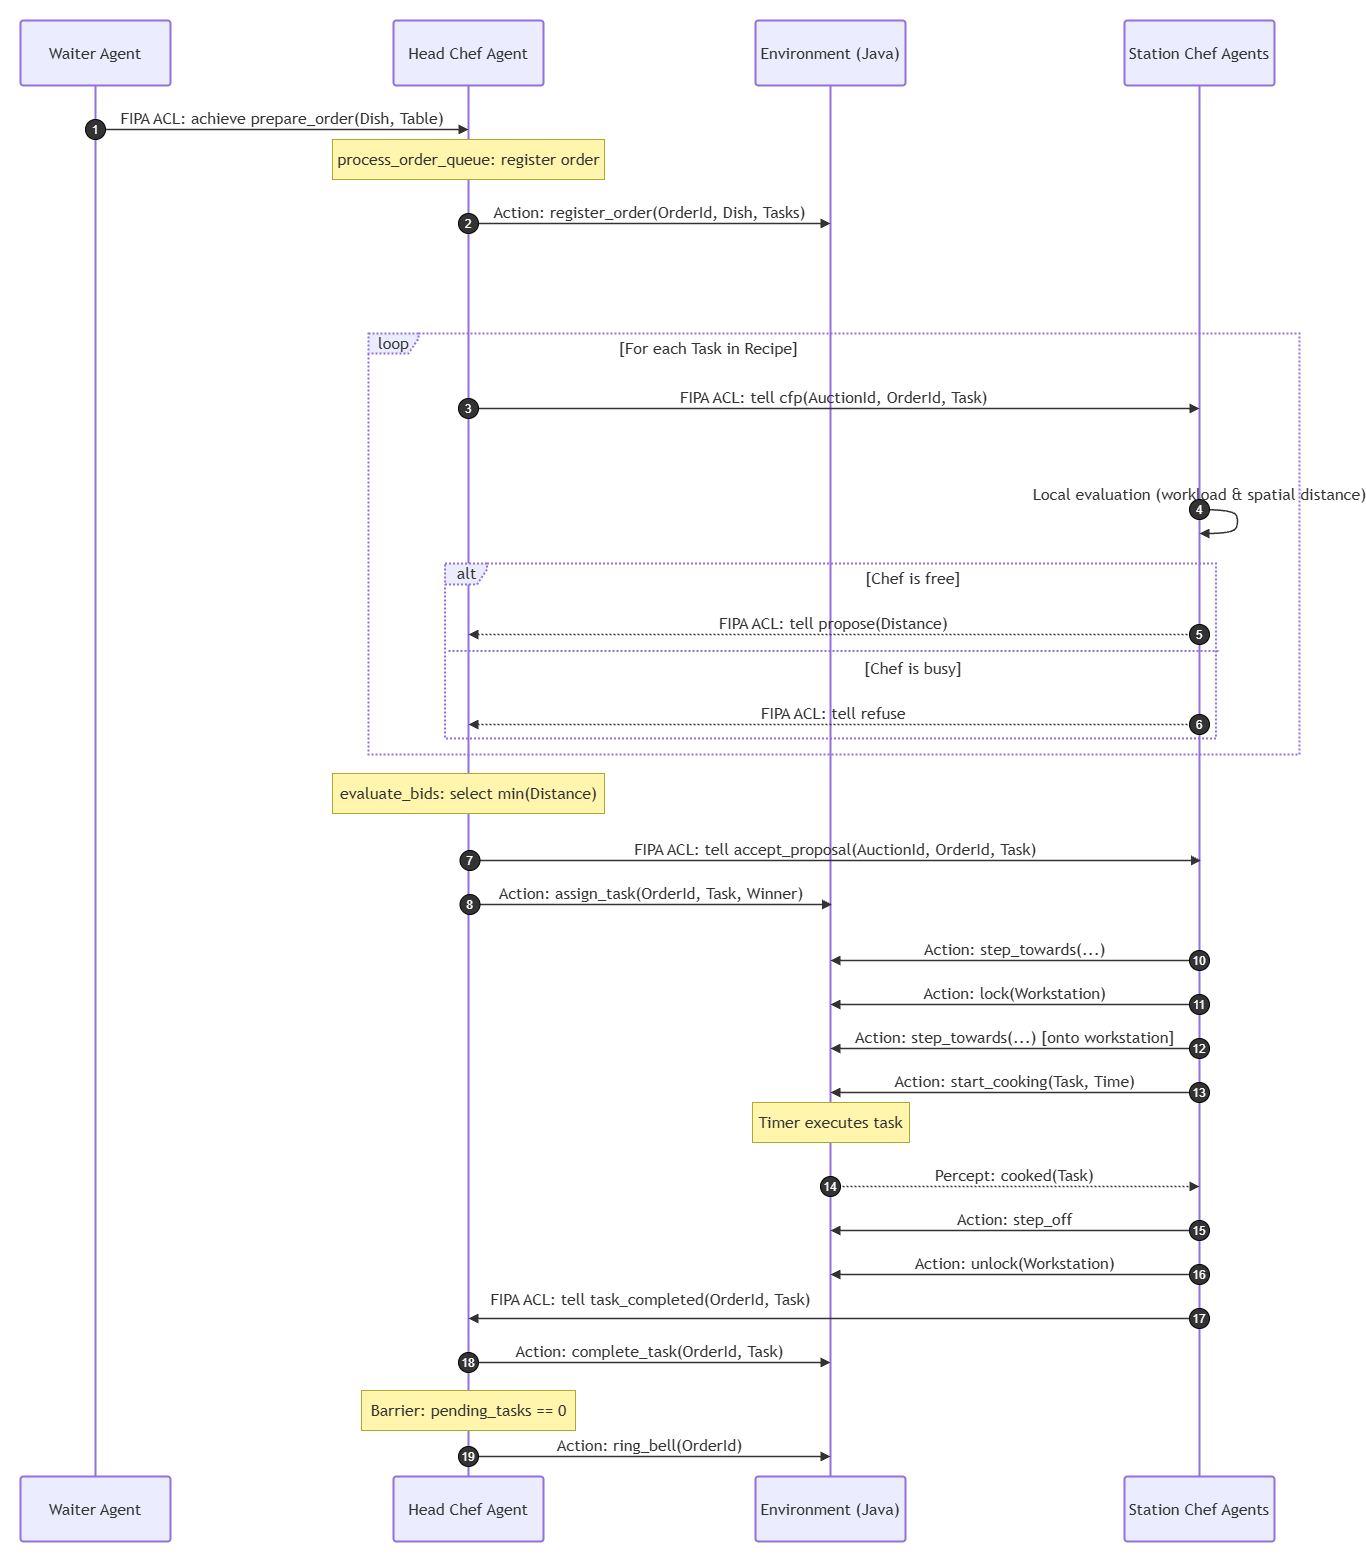
\includegraphics[width=0.8\textwidth]{assets/sequence-diagram_order-lifecycle.png}
    \caption{Sequence Diagram of the Order and Task Lifecycle.}
    \label{fig:class-diagram}
\end{figure}


\newpage
\section{The Environment}

In a MAS system an agent does not operate in isolation; it is inherently situated within an environment from which it receives percepts and inside which it executes actions. In ChefSync, the environment is engineered as a robust, first-class entity implemented in Java 21. It serves as the physical reality of the simulation, enforcing deterministic spatial and physical constraints that the cognitive layer cannot bypass.

This section details the concrete mechanics of the physical layer, including its spatial representation, temporal structure, concurrency control mechanisms, and user-facing observability infrastructure.

\subsection{Spatial and Temporal Model}

The physical boundaries of the kitchen are modeled as a discrete \textbf{2D Spatial Grid} consisting of distinct coordinates (x, y). Every operational entity within the system—including autonomous agents, prep counters, and specialized workstations—is assigned a specific spatial locus within this coordinate system.

\subsubsection{Spatial Constraints and Navigation}
The grid imposes strict physical laws on the system:
\begin{itemize}
\item \textbf{Cell Occupancy:} Workstations are static grid obstacles that agents cannot pass through unless they own the lock on that specific workstation. Other agents are treated as dynamic obstacles, preventing overlap.
\item \textbf{Movement Cost:} Pathfinding and movement require physical effort over time. For an agent to move, it must execute sequential \texttt{step\_towards} actions, shifting its coordinates one cell at a time. These movements are paired with logical pauses (e.g., \texttt{.wait} directives in the plans), introducing realistic temporal delays to the execution.
\end{itemize}

\subsubsection{Asynchronous, Event-Driven Execution}
ChefSync features a real-time, asynchronous, event-driven temporal model:
\begin{itemize}
\item \textbf{Real-Time Timers:} Physical processes (such as cooking a task on a workstation) are mapped to continuous real-world time. When an agent invokes \\texttt{start\_cooking(Task, Time)}, the physical layer starts an asynchronous Java \\texttt{TimerTask} that runs for the specified duration in milliseconds.
\item \textbf{Event-Driven Perceptions:} Upon timer expiration, the workstation state is mutated to register the completed task. The model then triggers a callback to the environment interface, invoking \\texttt{informAgsEnvironmentChanged()}. This notifies the Jason framework to perform a new reasoning cycle and update the agent's percepts (e.g., adding the \\texttt{cooked(Task)} belief), coupling the physical and logical layers asynchronously.
\end{itemize}

\subsection{Concurrency Control \& Resource Mutual Exclusion}

One of the core challenges addressed by the physical layer is the management of shared, finite hardware resources under high concurrency. Workstations such as Ovens, Grills, and Assembly Counters represent critical sections in the simulation. 

Because multiple Station Chef agents operate concurrently within the same physical space, unmanaged access to these workstations would inevitably cause state corruption or overlapping task execution. To prevent this, the physical layer implements strict \textbf{Mutual Exclusion (Mutex)} principles:

\begin{enumerate}
\item \textbf{Hardware-Level Locking:} Each workstation encapsulates a lock state (Unlocked vs. Locked by a specific agent) backed by thread-safe synchronization within the \\texttt{Workstation} model.
\item \textbf{Proximity-Constrained Locking Actions:} An agent must be adjacent to a workstation (distance less than or equal to 1 cell) to execute the \texttt{lock(Station)} action. Once the lock is successfully acquired, the agent is allowed to step onto the workstation cell to initiate cooking. If a Station Chef attempts to lock an already occupied resource, the environment rejects the action (returning \texttt{false} to the interpreter), which triggers the agent's BDI retry plan.
\item \textbf{Decoupled Error Handling:} Enforcing resource constraints at the environment model level rather than trusting agent behavior ensures safety. If an agent's social coordination fails (e.g., overlapping attempts), the physical model blocks illegal access, forcing the BDI reasoner to handle execution failures.
\end{enumerate}

\subsection{The Perception-Action Interface (\texttt{KitchenEnv})}

The connection between the Java physical layer and the Jason/AgentSpeak(L) logical layer is bridged by extending the core Jason \\texttt{Environment} class through \\texttt{KitchenEnv}. This component acts as a bidirectional translator, mapping semantic agent decisions into concrete object-oriented state mutations, and mapping physical states back into logical beliefs.

\subsubsection{Action Translation}
When an agent selects an action from its active intention stack, the Jason interpreter passes the term to \\texttt{KitchenEnv.executeAction()}. The environment inspects the functor, validates permissions based on the agent's assigned role, and invokes the underlying model methods:

\begin{itemize}
\item \textbf{Movement:}
\begin{itemize}
  \item \texttt{step\_towards(X, Y)}: Moves the agent one step closer to the destination.
  \item \texttt{step\_off}: Moves the agent off a workstation to a free adjacent cell.
\end{itemize}

\item \textbf{Resource Management:}
\begin{itemize}
  \item \texttt{lock(Station)}: Acquires an exclusive lock on a workstation.
  \item \texttt{unlock(Station)}: Releases the active workstation lock and clears completed tasks.
\end{itemize}
  
\item \textbf{Execution:}
\begin{itemize}
  \item \texttt{start\_cooking(Task, Time)}: Initiates an asynchronous timed cooking process on the occupied workstation.
\end{itemize}
  
\item \textbf{Orchestration (Head Chef only):}
\begin{itemize}
  \item \texttt{register\_order(OrderId, Dish, Tasks)}: Injects a new order and its sub-tasks into the dashboard.
  \item \texttt{assign\_task(OrderId, Task, Winner)}: Updates task assignment on the dashboard.
  \item \texttt{complete\_task(OrderId, Task)}: Marks a task as completed on the dashboard.
  \item \texttt{ring\_bell(OrderId)}: Completes the order status.
\end{itemize}
\end{itemize}

\subsubsection{Percept Generation}
At the beginning of each reasoning cycle, the environment updates the agents' belief bases by injecting localized \textbf{Percepts} via \texttt{KitchenEnv.getPercepts()}. The environment delivers:

\begin{itemize}
\item \texttt{kitchen\_status(open)}: Evaluates if the kitchen environment is operational.
\item \texttt{workstation(Name, X, Y)}: Static positions of all workstations.
\item \texttt{at(AgentName, X, Y)}: Dynamic coordinates of registered agents.
\item \texttt{cooked(Task)}: A localized, agent-specific perception indicating that the cooking timer for a task has completed on the workstation currently occupied by the calling agent.
\end{itemize}

\textit{Note: Workstation lock statuses are not broadcasted as percepts; mutual exclusion is managed via the return values of lock actions, and agents detect cell occupancy by reading the positions of other agents.}


\subsection{System Observability: Swing Visual Monitor}

To verify the correct execution of the Multi-Agent System and ensure full transparency, the environment incorporates a visualization framework implemented via \textbf{Java Swing} (\texttt{KitchenViewImpl}).

Following a strict separation of presentation and logic, the visual monitor operates as a pure observer of the underlying \texttt{KitchenModel}. It renders:
\begin{itemize}
\item \textbf{The 2D Grid Visualizer:} Displays real-time agent movements and workstation highlights (color-coded green for unlocked and red for locked, along with lock ownership labels).
\item \textbf{The Order \& Task Management Dashboard:} A side panel featuring a table that displays the order history and real-time task completion breakdown (showing task names, assignments, and completion states).
\end{itemize}

Because the view contains zero business logic and does not influence scheduling, it provides a clear window into the simulation without introducing side effects or affecting the timing of the BDI logic.


\newpage
\section{Multi-Agent System: BDI Logic \& Interaction}

The logical layer of ChefSync represents the cognitive "Mind" of the orchestrator. It is implemented using \textbf{Jason}, an interpreter for an extended version of the \textbf{AgentSpeak(L)} programming language. This architecture encapsulates control within autonomous entities that act proactively based on their internal mental states (Beliefs, Desires, and Intentions).

This section explores the specific roles assigned to the agents within the brigade, detailing their individual reasoning cycles and how they handle environmental unpredictability and execution failures.

\subsection{Agent Roles \& Reasoning}

The system's intelligence is distributed across three specialized agent roles. Each role is designed with a specific set of initial beliefs and plans, allowing the emergence of complex, coordinated behavior.

\subsubsection{The Waiter Agent: Asynchronous Demand Ingestion}
In a professional kitchen, the arrival of orders is asynchronous and outside the control of the cooking brigade. The \textbf{Waiter Agent} models this unpredictable workload.
\begin{itemize}
\item \textbf{Behavior:} The Waiter is programmed to simulate dining table events by asynchronously generating orders (macro-goals) and delegating them to the kitchen staff.
\item \textbf{Interaction:} It uses the FIPA ACL \texttt{achieve} performative to send a \texttt{prepare\_order(Dish, Table)} request directly to the Head Chef. By using the \texttt{achieve} act (which requests the receiver to adopt a goal) rather than a simple \texttt{tell} (which just updates a belief), the Waiter delegates the entire goal of preparing the dish, abstracting the physical fulfillment details.
\end{itemize}

\subsubsection{The Head Chef Agent: Coordination \& Barrier Synchronization}
The \textbf{Head Chef} acts as the central coordinator and planner of the brigade. It holds the cognitive responsibility of decomposing complex recipes and managing the order lifecycle.
\begin{itemize}
\item \textbf{Recipe Ontology:} The Head Chef's Belief Base is initialized with a menu ontology (\texttt{recipe(DishName, TaskList)}). When the Waiter delegates a goal, the addition event \texttt{+!prepare\_order(Dish, Table)} triggers the main planning process.
\item \textbf{Task Decomposition:} The Head Chef resolves the recipe to decompose the macro-goal (the dish) into a flat list of atomic, parallelizable sub-tasks (e.g., \texttt{grill\_patty}, \texttt{toast\_bun}, \texttt{assemble\_burger}).
\item \textbf{ContractNet Initiation:} The Head Chef initiates the ContractNet Protocol (CNP). It performs a directory facilitator search (\texttt{.df\_search}) for agents registered with the \texttt{station\_chef} role and issues a \textbf{multicast} Call for Proposal (CFP) to that specific group of candidates.
\item \textbf{Workstation Claiming:} When a Station Chef is awarded a task, it issues a \textbf{broadcast} message (\texttt{claiming(OrderId, Station)}) to all other agents in the platform, allowing peer-to-peer cognitive coordination to avoid workstation conflicts before physical navigation starts.
\item \textbf{Barrier Synchronization:} The Head Chef acts as a synchronization barrier. It maintains order completion state via the \texttt{pending\_tasks(OrderId, Dish, Table, Remaining)} belief. Every completed task decrements this count. When the remaining task count reaches zero, the Head Chef triggers the \texttt{ring\_bell(OrderId)} action in the environment to finalize the order.
\end{itemize}

\subsubsection{The Station Chef Agents: Spatial Navigation \& Failure Recovery}
The \textbf{Station Chef Agents} represent the autonomous workforce. They evaluate task proposals, coordinate their movements physically, and recover from failures in a highly concurrent environment.
\begin{itemize}
\item \textbf{Negotiation (Bid Evaluation):} Upon receiving a \texttt{cfp(AuctionId, OrderId, Task)}, a Station Chef evaluates its local commitments (\texttt{workload} and \texttt{pending\_bids}). If free, it computes a bid based on its Manhattan distance to the workstation required for that task, replying with a \texttt{propose(Bid)} FIPA ACL message.
\item \textbf{Spatial Navigation:} Once awarded a task (\texttt{accept\_proposal}), the agent executes a plan to reach the workstation coordinates. It issues sequential \texttt{step\_towards} actions in the environment, which uses a localized greedy heuristic to step closer while avoiding collision with other agents.
\item \textbf{Proximity Locking:} Upon reaching the destination, the agent must be adjacent to the workstation to execute the \texttt{lock(Station)} action. Once locked, it steps onto the station, executes \texttt{start\_cooking(Task, Time)}, waits for the environment percept \texttt{cooked(Task)}, steps off, and unlocks the workstation.
\item \textbf{BDI Fallback \& Recovery:} If movement or lock acquisition fails (due to congestion, lock contention, or equipment breakdown), the BDI engine triggers a plan failure handler: \texttt{-!perform\_task(AuctionId, OrderId, Task, Attempts)}. The agent increments its attempt counter and retries after a random delay. If the attempts exceed \texttt{max\_attempts}, it aborts and notifies the Head Chef by sending a \texttt{task\_failed(OrderId, Task)} message, triggering a re-auction of the task.
\end{itemize}

\subsection{FIPA ContractNet Protocol (CNP) Implementation}

The distribution of cooking tasks in ChefSync is dynamically negotiated using a FIPA-compliant ContractNet Protocol (CNP). This ensures that task allocation is not hardcoded, but emerges at runtime based on the state of the system.

\subsubsection{The Negotiation Process}

The protocol is divided into distinct phases involving the Head Chef (as the \textbf{Initiator}) and the Station Chefs (as the \textbf{Participants}):

\begin{enumerate}
\item \textbf{Call for Proposal (CFP):} The Head Chef launches an asynchronous intention (\\texttt{!start\_asynchronous\_auction}) for a specific task. It queries the Directory Facilitator to find the active Station Chefs and sends a multicast \texttt{cfp(AuctionId, OrderId, Task)} message. The Head Chef then waits for a deterministic timeout (e.g., 1.5 seconds) to allow participants to reply.
   
\item \textbf{Propose or Refuse:} Station Chefs receive the CFP and evaluate it. Based on their local state, they reply either with a \texttt{propose(Bid)} containing a heuristic cost score, or a \texttt{refuse} message.

\item \textbf{Evaluation \& Award:} Once the timeout expires, the Head Chef collects all proposals using \texttt{.findall}.
\begin{itemize}
   \item \textbf{Success Case:} If proposals are received, the Head Chef selects the optimal proposal using \texttt{.min}. It sends \texttt{accept\_proposal} to the winner, updates the physical dashboard via \texttt{assign\_task}, and sends \texttt{reject\_proposal} to the remaining bidders.
   \item \textbf{Failure/Retry Case:} If no proposals are received (e.g., all chefs are busy or workstations are contested), the Head Chef waits for a short period and spawns a retry auction.
\end{itemize}   
\end{enumerate}


\subsubsection{Utility \& Heuristic Evaluation Function}

To decide whether to bid and how to calculate the cost, the Station Chefs evaluate the incoming CFP against their local cognitive and physical context:

\paragraph{Cognitive Concurrency Gate}
Before calculating a bid, the Station Chef validates its capacity. To prevent resource over-commitment, an agent will only bid if it is completely free:
\begin{lstlisting}text
workload == 0  AND  pending_bids == 0
\end{lstlisting}
If the chef is currently cooking a task (\texttt{workload > 0}) or waiting for the outcome of another auction (\texttt{pending\_bids > 0}), it replies with a \texttt{refuse}.

\paragraph{Physical Contention Gate}
The agent checks if the workstation required for the task is already occupied by another agent or has been claimed by a peer at the cognitive level:
\begin{lstlisting}text
Occupied(Station)  OR  Claimed(Station)
\end{lstlisting}
If the workstation is unavailable, the chef refuses to prevent spatial conflicts and lock contention.

\paragraph{Heuristic Utility Score}
If both gates are passed, the chef computes a cost score based on spatial distance. Since moving through the grid takes time and steps, the utility of a task is inversely proportional to the distance:
\begin{lstlisting}text
Manhattan_Distance = |X_chef - X_station| + |Y_chef - Y_station|
\end{lstlisting}
The calculated \texttt{Bid} represents the Manhattan distance (total grid step actions required to reach the destination). The Head Chef's minimization function (\texttt{min}) naturally awards the task to the closest available chef, minimizing movement latency and maximizing kitchen throughput.

To guarantee encapsulation and high software modularity, the calculation is delegated to a \textbf{custom Java Internal Action} (\texttt{utils.calculate\_distance}). By decoupling this heuristic from the AgentSpeak plan logic, the distance calculation remains easily customizable for the future.


\newpage
\section{Implementation Details \& Tech Stack}

Translating the conceptual Multi-Agent System into a concrete, reproducible software requires a robust technology stack and a strictly organized codebase. This section outlines the core implementation decisions, the specific technologies adopted, and the structural organization of the ChefSync repository.

\subsection{Physical Layer Details}

\paragraph{Physical Model \& State Management}
At the core of the physical layer, the state of orders and tasks is managed by \texttt{KitchenModelImpl}. Because multiple agent threads and the Swing UI thread access and mutate this state concurrently, thread safety and structural clarity are enforced via:

\begin{itemize}
\item \textbf{Concurrent Data Structures:} The active orders are stored in a \texttt{ConcurrentHashMap<Integer, OrderRecord>} to prevent concurrency issues during concurrent reads and writes from the agent threads.

\item \textbf{Data Transfer Objects (Records):} To clean up data representation, order and task details are modeled as Java records. Records provide a concise syntax for data carriers, facilitating structured updates and state transfers:
\begin{lstlisting}[basicstyle=\footnotesize\ttfamily, breaklines=true]
public record TaskRecord(String name, String assignedTo, boolean completed) {}
public record OrderRecord(int id, String dish, String status, List<TaskRecord> tasks) {}
\end{lstlisting}

\item \textbf{Functional-Style State Replacement:} State transitions (like assigning a task or marking it complete) are performed by atomically replacing the existing record in the map with a newly instantiated record using stream mapping:
\begin{lstlisting}[basicstyle=\footnotesize\ttfamily, breaklines=true]
@Override
public void assignTask(int orderId, String task, String chef) {
  orders.computeIfPresent(orderId, (id, order) -> {
      List<TaskRecord> updated = order.tasks().stream()
          .map(t -> t.name().equals(task) ? new TaskRecord(t.name(), chef, t.completed()) : t)
          .collect(Collectors.toList());
      return new OrderRecord(id, order.dish(), order.status(), updated);
  });
  if (customView != null) customView.updateView();
}
\end{lstlisting}
\end{itemize}


\paragraph{Asynchronous Resource Execution (Cooking Timers)}
Culinary execution requires physical time. Instead of blocking the agent's main execution thread during cooking (which would freeze the BDI reasoning loop), the environment delegates cooking tasks to background timers:

\begin{itemize}
\item \textbf{Timer Delegation:} When a Station Chef agent invokes the \texttt{start\_cooking(Task, Time)} action, the \texttt{WorkstationImpl} schedules a \texttt{java.util.TimerTask}:
\begin{lstlisting}[basicstyle=\footnotesize\ttfamily, breaklines=true]
public synchronized void startCooking(String task, int timeMs, Runnable onComplete) {
  this.completedTask = null;
  timer.schedule(new TimerTask() {
      @Override
      public void run() {
          synchronized (WorkstationImpl.this) {
              completedTask = task;
          }
          if (onComplete != null) onComplete.run();
      }
  }, timeMs);
}
\end{lstlisting}

\item \textbf{Decoupled Notification \& Asynchronous Repainting:} Once the timer expires, the workstation updates its state and executes the \texttt{onComplete} callback. This callback does two things: it triggers the asynchronous repainting of the Swing GUI to keep the visual monitor updated, and it invokes \texttt{informAgsEnvironmentChanged()}. This signals the Jason interpreter to perform a new reasoning cycle and update the agent's percepts, adding the belief \texttt{cooked(Task)} so the agent can resume its plan.
\end{itemize}


\subsection{Technology Stack}

The project relies on a modern, standard toolchain designed to guarantee cross-platform execution, ease of integration, and reproducibility without relying on specific IDE configurations:

\begin{itemize}
\item \textbf{Java 21 (LTS):} Serves as the foundational programming language for the physical environment, the concurrent data structures, and the Swing GUI. The choice of Java 21 allows the use of modern language features while ensuring long-term support and high performance for the real-time asynchronous execution and thread-safe operations.
\item \textbf{Jason 3.2.1:} The core BDI framework. It acts as the interpreter for the AgentSpeak(L) language. Rather than relying on legacy or unstable IDE plugins, Jason is integrated as a library dependency, allowing it to be seamlessly booted and managed programmatically.
\item \textbf{Gradle:} Used as the build automation and dependency management tool. By providing a Gradle Wrapper (\texttt{gradlew}), the project guarantees full reproducibility. The MAS can be built, tested, and run from the command line without needing to manually configure Jason classpaths or install additional software.
\end{itemize}


\subsection{Repository Structure}

To enforce the Separation of Concerns (SoC), the source code strictly separates the cognitive "Mind" from the physical "Body" using a footprint directory layout:

\begin{itemize}
\item \textbf{\texttt{src/main/asl/} (The Mind):} This directory encapsulates the cognitive layer. It contains all the AgentSpeak source files (\texttt{.asl}) that define the beliefs, plans, and reasoning cycles of the agents (\texttt{waiter.asl}, \texttt{head\_chef.asl}, \texttt{station\_chef.asl}).

\item \textbf{\texttt{src/main/java/} (The Body):} This directory encapsulates the physical and infrastructural layers. It is further modularized following a Model-View-Controller (MVC) inspired pattern:
\begin{itemize}
  \item \texttt{env/}: Contains the \texttt{KitchenEnv.java} bridge that translates AgentSpeak actions into Java methods and generates percepts.
  \item \texttt{model/}: Contains the core business logic of the simulation, including the \texttt{KitchenModel}, \texttt{Workstation} locks, and spatial tracking.
  \item \texttt{view/}: Contains the Java Swing components (\texttt{KitchenView}) responsible for passively rendering the state of the model.
  \item \texttt{utils/}: Contains custom internal actions and utility helper classes (such as \texttt{calculate\_distance.java}) that extend the AgentSpeak language capabilities.
\end{itemize}

\item \textbf{\texttt{src/test/}:} Contains the JUnit suites for environment and E2E MAS integration testing.
\end{itemize}


\subsection{System Bootstrapping: \texttt{chefsync.mas2j}}

The entry point of the Multi-Agent System is the \texttt{chefsync.mas2j} configuration file. This file acts as the primary orchestrator for the Jason framework during the boot phase. Its role is fundamental for establishing the system boundaries:

\begin{enumerate}
\item \textbf{Environment Binding:} It explicitly links the logical MAS to the Java physical layer by declaring the custom environment class (\texttt{environment: env.KitchenEnv}).
\item \textbf{Agent Instantiation:} It defines the exact composition of the kitchen brigade, specifying which \texttt{.asl} files to compile and how many instances of each agent to spawn (e.g., spawning exactly one \texttt{head\_chef} but a dynamically configurable number of \texttt{station\_chef} agents).
\item \textbf{Infrastructure Management:} It configures the internal Jason infrastructure (using the Centralised infrastructure) and manages the classpath mappings required to bridge the \texttt{.asl} files with the compiled Java classes.
\end{enumerate}


\newpage
\section{Testing, Validation \& Reproducibility}

Validating a decentralized system of autonomous agents presents unique challenges compared to standard procedural software, as the control flow is non-deterministic and emerges from asynchronous social interactions. 

ChefSync addresses this by combining isolated unit testing of the physical layer, automated End-to-End (E2E) integration testing of the Multi-Agent System (MAS), and real-time observability of spatial and social dynamics.

\subsection{Unit Testing (Physical Layer Validation)}

Before evaluating the cognitive coordination of the agents, the physical layer must be proven correct. Because the Java codebase enforces the rules of the simulation, the project includes isolated unit tests using JUnit to validate the model and environment controller in isolation.

\subsubsection{Model State \& Rules Verification (\texttt{KitchenModelTest})}
The spatial and resource constraints are validated in the \texttt{KitchenModelTest} suite. These tests ensure the simulation's integrity:
\begin{itemize}
\item \textbf{Spatial Constraints:} Verifies coordinate bounds, grid positioning, and that agents cannot occupy cells occupied by other agents.
\item \textbf{Workstation Mutex Locks:} Validates that a workstation can only be locked by one agent at a time, and that locking is proximity-restricted (the locking agent must be adjacent).
\item \textbf{Order \& Task State Tracking:} Verifies that orders and their sub-tasks are correctly registered, assigned to chefs, and marked as completed, ensuring that the model updates and tracks state transitions properly.
\end{itemize}

\subsubsection{Environment Bridge \& RBAC Validation (\texttt{KitchenEnvTest})}
The gateway connecting the agents to the environment is validated in \texttt{KitchenEnvTest}. These tests focus on action parsing and security:
\begin{itemize}
\item \textbf{Role-Based Access Control (RBAC):} Verifies that only authorized agent roles can execute specific actions (e.g., verifying that a \texttt{station\_chef} is blocked from executing \texttt{register\_order}, while the \texttt{head\_chef} is allowed).
\item \textbf{Action Execution Translation:} Assures that AgentSpeak actions are correctly parsed, mapped to the correct model calls, and return the correct boolean status to the agent interpreter.
\end{itemize}


\subsection{End-to-End (E2E) Integration Testing}

To programmatically verify the emergent behavior of the brigade, the project includes an automated test suite built with JUnit 4. The core of this suite is the \\texttt{ChefsyncEndToEndTest}, which evaluates the entire Multi-Agent System lifecycle without requiring human intervention.

\subsubsection{Headless MAS Execution}
Instead of launching the Jason MAS with its graphical Swing interface, the JUnit test utilizes the \texttt{RunLocalMAS} wrapper to boot the Jason infrastructure in \textbf{headless mode}. This allows the test suite to programmatically instantiate the \texttt{chefsync.mas2j} configuration within a Continuous Integration (CI) environment.

\subsubsection{Synchronization Latch (\texttt{testLatch})}
To bridge the JUnit runner thread with the asynchronous Jason agent threads without consuming CPU cycles in polling loops, the environment includes a synchronization hook:
\begin{itemize}
\item A static \texttt{CountDownLatch} (\texttt{testLatch}) is initialized by JUnit before starting the MAS.
\item When the Head Chef successfully completes the first order (invoking the \texttt{ring\_bell} action), the environment decrements the latch (\texttt{testLatch.countDown()}), instantly waking up the JUnit thread.
\end{itemize}

\subsubsection{E2E Integration Assertions}
The test verifies the full, unbroken chain of events:
\begin{enumerate}
\item \textbf{Bootstrapping:} Checks that all agents (Waiter, Head Chef, Station Chefs) spawn and register.
\item \textbf{Social Interaction:} Verifies that the Waiter sends the order request, the Head Chef decomposes the recipe, and the Station Chefs dynamically negotiate via FIPA ACL.
\item \textbf{Physical Action Integration:} Verifies that chefs successfully navigate the grid, lock the workstations, cook, and notify completion.
\item \textbf{Safety \& Liveness:} Confirms the order completes within the 45-second safety timeout, asserting that the system is free of deadlocks and logical stalls.
\end{enumerate}


\subsection{Continuous Integration (GitHub Actions)}

To ensure that modifications to the agents or the environment code do not break existing functionality or introduce new bugs, the repository integrates a Continuous Integration (CI) pipeline using \textbf{GitHub Actions}. On every \texttt{push} or \texttt{pull\_request} to the \texttt{main} and \texttt{develop} branches, a workflow compiles the code under JDK 21 and runs the complete test suite. Because the physical environment utilizes Swing GUI components, the workflow wraps the test execution command with \texttt{xvfb-run} to virtualize the display environment and allow headless UI-bound test execution in the CI runner.


\subsection{Visual and Console Validation}

While automated tests ensure structural correctness, manual and visual validation remains essential for analyzing the complex social dynamics and spatial heuristics of the agents.

\subsubsection{Social \& Log Traceability}

To monitor the cognitive coordination and internal states of the agents, the system provides two distinct debugging interfaces:

\begin{itemize}
\item \textbf{Jason MAS Console (GUI):} A Swing-based console window automatically spawned by the Jason framework at startup. It aggregates the stdout logs, logging outputs, and \texttt{.print} instructions from all active agents into a single centralized view. It also provides basic controls (such as pause, resume, and stop) to inspect the execution flow step-by-step.
\item \textbf{Agent Mind Inspector (Web Interface):} Jason hosts a local web server running the Mind Inspector. This web interface allows evaluators to inspect the internal BDI state of any agent dynamically. It shows their active belief base (e.g., current position, held locks, claims), active desires (goals), and the exact execution stack of their current intentions.
\end{itemize}

\subsubsection{Spatial Validation (The Swing GUI)}
Simultaneously, the Swing GUI provides a passive window into the physical consequences of those cognitive decisions. It allows the user to visually validate:
\begin{itemize}
\item \textbf{Spatial Coordination:} Observing the Station Chefs physically moving step-by-step across the grid, confirming that they avoid static obstacles and dynamically choose the shortest path using the model's greedy Manhattan distance minimization heuristic.
\item \textbf{Concurrency Safety:} Observing the color-coded workstation locks (green/red), ensuring that no two agents ever occupy or cook at the same critical hardware resource simultaneously.
\item \textbf{Order Tracking Panel:} Monitoring the real-time table, validating that order states and task assignment progress update immediately in response to execution events.
\end{itemize}
\clearpage


\newpage
\section{Deployment \& Execution}

This chapter provides step-by-step, reproducible instructions to build, execute, and validate the ChefSync Multi-Agent System on different operating systems.


\subsection{Prerequisites}
To run the simulation and compile the codebase, the host environment must satisfy the following minimal requirements:
\begin{itemize}
\item \textbf{Java Development Kit (JDK):} Version \textbf{21} or higher must be installed and properly configured in the system's path.
\end{itemize}

\textit{Note: No local installation of Gradle is required, as the project includes the Gradle Wrapper (\texttt{gradlew} / \texttt{gradlew.bat}).}


\subsection{Clone the Repository}
Clone the project from the version control system and navigate into the root directory:
\begin{lstlisting}[basicstyle=\footnotesize\ttfamily, breaklines=true]
git clone https://github.com/GiorgioFantilliUnibo/chefsync-mas.git
cd chefsync-mas
\end{lstlisting}

\subsection{Executing the Multi-Agent System}
To launch the Multi-Agent System (which boots the Swing visual monitor, the Jason MAS Console, and spawns the Waiter, Head Chef, and Station Chef agents), execute the custom Gradle task:

\paragraph{On Linux / macOS:}~\\
\begin{lstlisting}[basicstyle=\footnotesize\ttfamily, breaklines=true]
./gradlew runChefsyncMas
\end{lstlisting}

\paragraph{On Windows:}~\\
\begin{lstlisting}[basicstyle=\footnotesize\ttfamily, breaklines=true]
.\gradlew.bat runChefsyncMas
\end{lstlisting}

\paragraph{Expected Output \& Interfaces}
Once the boot phase completes, the following components will launch automatically:
\begin{enumerate}
\item \textbf{The Visual Monitor (Java Swing GUI):} Renders the 2D grid depicting workstations and chefs moving in real-time, side-by-side with the \textit{Order \& Task Management} dashboard JTable tracking order states.
\item \textbf{The Jason MAS Console:} Spawns a Java Swing window showing aggregated real-time agent output prints and coordination logs, with buttons to pause, step, or stop execution.
\end{enumerate}


\subsection{Running Automated Tests}

To execute the entire test suite—including the physical layer unit tests (\texttt{KitchenModelTest} and \texttt{KitchenEnvTest}) and the headless integration test (\texttt{ChefsyncEndToEndTest}):

\paragraph{On Linux / macOS:}~\\
\begin{lstlisting}[basicstyle=\footnotesize\ttfamily, breaklines=true]
./gradlew test
\end{lstlisting}

\paragraph{On Windows:}~\\
\begin{lstlisting}[basicstyle=\footnotesize\ttfamily, breaklines=true]
.\gradlew.bat test
\end{lstlisting}


\newpage
\section{Conclusions \& Future Work}

In conclusion, ChefSync successfully demonstrates how a multi-agent system can coordinate a busy restaurant kitchen. Using the BDI paradigm and the Jason framework, we modeled the kitchen staff as autonomous agents that can plan, react to orders, negotiate tasks via FIPA ContractNet, and handle execution failures dynamically.

The current implementation has some limits. Physical simulation calculations (such as coordinates and movement steps) are computed centrally in Java, which would slow down the simulation if we scaled up to a much larger kitchen. Additionally, agents must manage workstation locks and queue priorities cognitively by constantly exchanging beliefs and messages.

To improve this, a future development would be integrating the \textbf{Agents \& Artifacts (A\&A)} paradigm. Instead of custom Java models and direct communication for locking, workstations and order queues would be modeled as external "artifacts". Agents would interact with these artifacts indirectly (stigmergy) by reading their public properties and calling their operations (like \texttt{lock} or \texttt{cook}). This would simplify agent code, reduce communication overhead, and make the whole system much more modular and scalable.

\clearpage
\end{document}